%% article class — Overleaf-compatible replacement for Springer svjour3
\documentclass[11pt,a4paper]{article}
\usepackage[top=2.5cm,bottom=2.5cm,left=2.8cm,right=2.8cm]{geometry}

%% ── svjour3 compatibility layer ──────────────────────────────────────────────
%% These stubs replace Springer-specific macros so the document compiles
%% on any standard LaTeX installation / Overleaf without svjour3.cls.

\newcommand{\smartqed}{}          % QED symbol hook — no-op here
\newcommand{\journalname}[1]{}    % journal header — no-op
\newcommand{\titlerunning}[1]{}   % running title — no-op
\newcommand{\authorrunning}[1]{}  % running author — no-op
\newcommand{\inst}[1]{\textsuperscript{\normalfont\small#1}}
\newcommand{\email}[1]{\texttt{#1}}

%% \institute: store content, then display it right after \maketitle
\makeatletter
\gdef\@svjinstitute{}
\newcommand{\institute}[1]{\gdef\@svjinstitute{#1}}
\AtBeginDocument{%
  \let\svj@origmaketitle\maketitle
  \renewcommand{\maketitle}{%
    \svj@origmaketitle
    \ifx\@svjinstitute\@empty\else
      \begin{center}\small\let\and\par\@svjinstitute\end{center}%
      \vspace{-0.5em}%
    \fi
  }%
}
\makeatother

%% \keywords inside abstract: \and → "; "
\newcommand{\keywords}[1]{%
  \par\vspace{0.6em}\noindent\textbf{Keywords:}\enspace
  \begingroup\def\and{; }#1\endgroup\par%
}

%% acknowledgements environment
\newenvironment{acknowledgements}{%
  \section*{Acknowledgements}%
}{}
%%──────────────────────────────────────────────────────────────────────────────

%% ── Packages ─────────────────────────────────────────────────────────────────
\usepackage{graphicx}
\usepackage{amsmath,amssymb,bm}
\usepackage{tikz}
\usetikzlibrary{shapes.geometric,arrows.meta,positioning,fit,
                backgrounds,calc,decorations.pathreplacing}
\usepackage{pgfplots}
\pgfplotsset{compat=1.18}
\usepgfplotslibrary{colorbrewer}
\usepackage[ruled,vlined,linesnumbered]{algorithm2e}
\usepackage{booktabs}
\usepackage{multirow}
\usepackage{colortbl}
\usepackage{array}
\usepackage{xcolor}
\usepackage{subfig}
\usepackage{url}
\usepackage{cite}

%% ── Colour palette ───────────────────────────────────────────────────────────
\definecolor{structcol}{RGB}{70,130,180}    % steel blue
\definecolor{textcol}{RGB}{60,179,113}      % medium sea-green
\definecolor{evolcol}{RGB}{210,105,30}      % chocolate
\definecolor{gacol}{RGB}{147,112,219}       % medium purple
\definecolor{anncol}{RGB}{220,80,80}        % indian red
\definecolor{lightgray}{RGB}{240,240,240}

%% ── Journal metadata ─────────────────────────────────────────────────────────
\journalname{Engineering Applications of Artificial Intelligence}

%% ─────────────────────────────────────────────────────────────────────────────
\begin{document}

\title{A Hybrid Neuro-Genetic Framework for Automated Software%
        Maintainability Assessment Using Multidimensional Code Metrics}

\titlerunning{Hybrid Neuro-Genetic Framework for Software Maintainability}

\author{[Author~1]\inst{1} \and [Author~2]\inst{1} \and [Author~3]\inst{2}}
\authorrunning{[Author~et~al.]}

\institute{[Department, University, Country]\\\email{[author@institution.edu]}
\and
[Department, University, Country]}

\date{Received: [DD Month YYYY] / Accepted: [DD Month YYYY]}

\maketitle

%% ── Abstract ─────────────────────────────────────────────────────────────────
\begin{abstract}
Software maintenance accounts for a disproportionate share of total
lifecycle cost, yet automated, data-driven methods for assessing file-level
maintainability risk remain limited by two persistent deficiencies: reliance on
purely structural code metrics and manual, correlation-guided feature selection.
This paper presents a hybrid \emph{Neuro-Genetic Maintainability Framework}
that addresses both shortcomings simultaneously. The proposed system mines a
19-dimensional feature space partitioned into three orthogonal categories ---
\emph{Structural}, \emph{Textual}, and \emph{Evolutionary} --- extracted
from both static analysis and version-controlled Git history, providing richer
behavioural context than structural signals alone. A Genetic Algorithm (GA)
performs automated binary feature selection guided by a multi-objective fitness
function that jointly optimises predictive accuracy and feature parsimony,
eliminating the subjective threshold choices inherent in Pearson-correlation
filtering. An Artificial Neural Network (ANN), whose architecture is
pre-tuned via Bayesian optimisation (Optuna), serves as the fitness evaluator
within each generation. Snapshot-based data extraction enforces strict temporal
isolation, ensuring that no future-commit information contaminates training
labels. Experiments across three mature open-source Python repositories ---
Flask, Requests, and FastAPI --- demonstrate that the GA-selected subsets
achieve validation Mean Squared Errors of $0.139$, $0.220$, and $0.254$
respectively while reducing the feature space by 44--71\%. Across all
repositories, the GA consistently selects cross-dimensional subsets, validating
the hypothesis that structural complexity must be paired with developer-churn
and readability signals to accurately capture maintainability risk.
Sensitivity analysis confirms robustness of the fitness-weight hyperparameters
over a wide operating range.

\keywords{Software maintainability prediction \and Genetic algorithm \and
Artificial neural network \and Feature selection \and Code metrics \and
Evolutionary metrics \and Software engineering}
\end{abstract}

%% ─────────────────────────────────────────────────────────────────────────────
\section{Introduction}
\label{sec:intro}
%% ─────────────────────────────────────────────────────────────────────────────

The economic cost of software maintenance has long been understood to dominate
the total cost of ownership of large software systems~\cite{liHenry1993}.
Surveys consistently report that corrective and adaptive maintenance together
consume between 60\% and 80\% of a system's total lifecycle expenditure, with
the proportion rising as codebases grow in complexity~\cite{riaz2009systematic}.
A developer confronted with a large, unfamiliar repository faces the immediate
practical problem of identifying which files are most likely to require future
intervention --- a problem for which manual code review is neither scalable
nor reproducible.

Prediction models that associate measurable code properties with future
maintenance effort have consequently attracted sustained research interest since
the foundational work of Li and Henry~\cite{liHenry1993}, who demonstrated
that object-oriented design metrics from the Chidamber--Kemerer (CK) suite
correlate meaningfully with the number of lines changed per class. Subsequent
studies extended this line of inquiry through increasingly expressive machine
learning models, including artificial neural networks~\cite{vescan2025},
hybrid functional-link networks with evolutionary optimisation~\cite{kumarRath2016},
and ensemble methods~\cite{alsolai2019application}. Yet three limitations
have persisted across the majority of this literature.

\textbf{First}, feature spaces are almost universally confined to static,
structural metrics. Structural complexity captures the internal organisation
of code at a single moment in time but is silent about how that code has
evolved, who has modified it, and whether it has historically attracted
defect-related commits. Git-mined evolutionary metrics --- commit frequency,
author count, code churn, bug-fix ratio --- have been shown to be strong
independent predictors of defect density~\cite{nagappan2005use}, yet they are
rarely combined with static metrics in maintainability models.

\textbf{Second}, feature selection is typically performed by manually
thresholding Pearson correlation values~\cite{vescan2025}, a process that
is dataset-specific, requires human judgement, and optimises a univariate
criterion that cannot capture joint redundancy or synergy among features.

\textbf{Third}, temporal data integrity is seldom enforced. When metrics and
labels are extracted from the same historical window, information about future
bug-fix activity can leak into training features, producing optimistic evaluation
estimates that do not generalise to unseen code~\cite{dambros2012}.

This paper addresses all three limitations within a single, end-to-end
automated pipeline. Our contributions are as follows.

\begin{itemize}
  \item A \textbf{three-dimensional feature taxonomy} (Structural,
        Textual, Evolutionary) comprising 19 features mined jointly from
        static AST analysis and Git history, expanding the representational
        richness far beyond the CK-only baseline.
  \item A \textbf{GA-driven automated feature selection} mechanism that
        simultaneously minimises prediction error and maximises feature
        parsimony via a dual-objective fitness function, replacing manual
        correlation filtering with a principled combinatorial search.
  \item A \textbf{snapshot-based temporal isolation} protocol that defines
        the feature observation window and the label window as non-overlapping
        intervals in Git history, eliminating forward-looking data leakage.
  \item \textbf{Bayesian hyperparameter optimisation} (Optuna) of the ANN
        architecture, ensuring that the fitness evaluator is itself near-optimal
        before genetic search begins.
  \item An \textbf{empirical multi-repository evaluation} across Flask,
        Requests, and FastAPI, supplemented by ablation analysis, sensitivity
        sweeps, and statistical significance testing.
\end{itemize}

The remainder of this paper is structured as follows.
Section~\ref{sec:related} surveys related work. Section~\ref{sec:framework}
describes the proposed framework in full. Section~\ref{sec:setup} details the
experimental setup. Section~\ref{sec:results} presents results and answers the
research questions. Section~\ref{sec:discussion} discusses implications and
limitations. Section~\ref{sec:threats} addresses threats to validity. Section~\ref{sec:conclusion}
concludes.

%% ─────────────────────────────────────────────────────────────────────────────
\section{Related Work}
\label{sec:related}
%% ─────────────────────────────────────────────────────────────────────────────

\subsection{Metrics-Based Maintainability Prediction}

The CK metrics suite proposed by Chidamber and Kemerer~\cite{ck1994} --- including
Weighted Methods per Class, Depth of Inheritance Tree, Coupling Between Objects,
and Lack of Cohesion in Methods --- became the primary feature set for
object-oriented maintainability research. Li and Henry~\cite{liHenry1993} applied
these metrics in regression models on the UIMS and QUES datasets, establishing
a benchmark that subsequent work has repeatedly revisited. Elmidaoui
et al.~\cite{elmidaoui2019} conducted a systematic review of over 80 empirical
studies and found that design metrics dominate the literature, with dynamic and
process metrics significantly underrepresented.

Riaz et al.~\cite{riaz2009systematic} performed a systematic literature review
of maintainability prediction techniques and noted that change-based metrics
and the Maintainability Index are the two most commonly used proxy variables.
They identified a consistent gap: most studies operate on single projects and
do not examine how well the selected feature sets transfer to other codebases.
Our multi-repository design directly addresses this cross-project generalisability
concern.

\subsection{Machine Learning Approaches}

Kumar and Rath~\cite{kumarRath2015,kumarRath2016} proposed hybrid functional-link
ANN architectures combined with genetic algorithms, Particle Swarm Optimisation,
and Clonal Selection Algorithms, demonstrating improvements over linear regression
on the same UIMS/QUES datasets. Schnappinger et al.~\cite{schnappinger2019} trained
classifiers on tool-measured static analysis data from three Java projects, finding
that a decision tree achieved 80\% precision. Alsolai and Roper~\cite{alsolai2019application}
argued that ensemble methods are a promising future direction, though their paper
presented a research plan without empirical results. Gupta and Chug~\cite{gupta2021}
proposed an Optimised Extreme Learning Machine, outperforming several standard
classifiers on three open-source datasets.

The most directly related recent work is Vescan and Barac-Antonescu~\cite{vescan2025},
who introduced a Neural Network Change Prediction (NNCP) approach that applies
Pearson correlation to select a small subset of CK metrics as inputs to a
feed-forward ANN. Their Model~4, which considers only metrics correlated above
a project-specific threshold with the change metric, outperformed regression
and hybrid FLANN baselines on the QUES dataset. Our framework extends NNCP
in every dimension: automated feature selection, enriched feature space, temporal
isolation, and Bayesian hyperparameter tuning.

\subsection{Evolutionary Metrics and Git Mining}

The relationship between version-control history and software quality has been
studied independently of the maintainability prediction literature.
Nagappan and Ball~\cite{nagappan2005use} demonstrated that code churn --- the
cumulative volume of lines added, deleted, and modified --- is a reliable
predictor of post-release defect density in large Microsoft products.
Rahman and Devanbu~\cite{rahman2013} showed that process metrics derived from
commit history frequently outperform static code metrics in predicting failures,
a finding that motivates the inclusion of our Category~C evolutionary features.
Hassan~\cite{hassan2009predicting} used change complexity and entropy of code
changes to predict faults, while Zimmermann et al.~\cite{zimmermann2007} exploited
software network structure in version repositories. To our knowledge, no prior
maintainability prediction framework systematically combines structural, textual,
and evolutionary metrics within a single GA-driven feature selection loop.

%% ─────────────────────────────────────────────────────────────────────────────
\section{Proposed Framework}
\label{sec:framework}
%% ─────────────────────────────────────────────────────────────────────────────

\subsection{Architecture Overview}
\label{subsec:overview}

Figure~\ref{fig:pipeline} depicts the four-stage pipeline that constitutes
the Neuro-Genetic Maintainability Framework. The stages are executed
sequentially: \emph{Data Collection} mines raw metrics and labels;
\emph{Preprocessing} enforces integrity and normalisation;
\emph{Genetic Optimisation} evolves the optimal feature chromosome; and
\emph{Analysis} generates comparative, ablation, and statistical results.

%% ── Figure 1: Pipeline ───────────────────────────────────────────────────────
\begin{figure*}[!t]
\centering
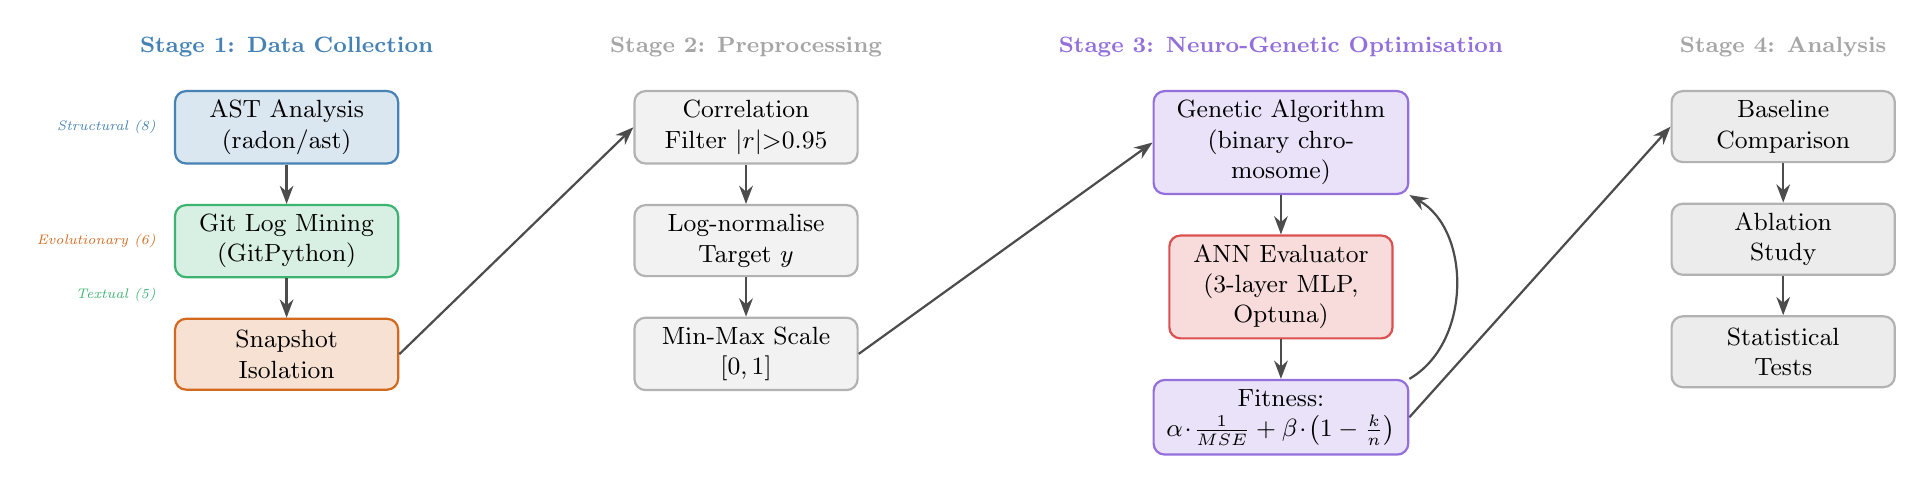
\begin{tikzpicture}[
  node distance=0.7cm and 1.5cm,
  box/.style={rectangle, rounded corners=4pt, minimum width=2.8cm,
               minimum height=0.9cm, align=center, text width=2.6cm,
               font=\small, draw=black!60, thick},
  sbox/.style={box, fill=structcol!20, draw=structcol},
  tbox/.style={box, fill=textcol!20,   draw=textcol},
  ebox/.style={box, fill=evolcol!20,   draw=evolcol},
  gabox/.style={box, fill=gacol!20,    draw=gacol, minimum width=3.2cm,
                text width=3.0cm},
  annbox/.style={box, fill=anncol!20,  draw=anncol},
  outbox/.style={box, fill=gray!15,    draw=gray!60},
  arr/.style={-Stealth, thick, draw=black!70},
  >=Stealth
]

%% Stage labels
\node[font=\bfseries\footnotesize, text=structcol] (s1lbl)
  {Stage 1: Data Collection};

%% Stage 1 boxes (vertical column)
\node[sbox, below=0.3cm of s1lbl] (ast)
  {AST Analysis\\(radon/ast)};
\node[tbox, below=0.5cm of ast] (git)
  {Git Log Mining\\(GitPython)};
\node[ebox, below=0.5cm of git] (snap)
  {Snapshot\\Isolation};

%% Stage 2
\node[font=\bfseries\footnotesize, text=gray!70, right=2.0cm of s1lbl]
  (s2lbl) {Stage 2: Preprocessing};
\node[box, fill=gray!10, draw=gray!60, below=0.3cm of s2lbl] (corr)
  {Correlation\\Filter $|r|{>}0.95$};
\node[box, fill=gray!10, draw=gray!60, below=0.5cm of corr] (log)
  {Log-normalise\\Target $y$};
\node[box, fill=gray!10, draw=gray!60, below=0.5cm of log] (scale)
  {Min-Max Scale\\$[0,1]$};

%% Stage 3 – GA+ANN
\node[font=\bfseries\footnotesize, text=gacol, right=2.0cm of s2lbl]
  (s3lbl) {Stage 3: Neuro-Genetic Optimisation};
\node[gabox, below=0.3cm of s3lbl] (ga)
  {Genetic Algorithm\\(binary chromosome)};
\node[annbox, below=0.5cm of ga] (ann)
  {ANN Evaluator\\(3-layer MLP, Optuna)};
\node[gabox, below=0.5cm of ann] (fit)
  {Fitness:\\$\alpha\!\cdot\!\frac{1}{MSE}+\beta\!\cdot\!\bigl(1-\tfrac{k}{n}\bigr)$};

%% Stage 4
\node[font=\bfseries\footnotesize, text=gray!70, right=2.0cm of s3lbl]
  (s4lbl) {Stage 4: Analysis};
\node[outbox, below=0.3cm of s4lbl] (bl)   {Baseline\\Comparison};
\node[outbox, below=0.5cm of bl]    (abl)  {Ablation\\Study};
\node[outbox, below=0.5cm of abl]   (stat) {Statistical\\Tests};

%% Arrows within stages
\draw[arr] (ast) -- (git);
\draw[arr] (git) -- (snap);
\draw[arr] (corr) -- (log);
\draw[arr] (log) -- (scale);
\draw[arr] (ga)  -- (ann);
\draw[arr] (ann) -- (fit);
\draw[arr] (fit.north east) to[out=30,in=-30] (ga.south east);
\draw[arr] (bl) -- (abl);
\draw[arr] (abl) -- (stat);

%% Cross-stage arrows
\draw[arr] (snap.east) -- (corr.west);
\draw[arr] (scale.east) -- (ga.west);
\draw[arr] (fit.east)  -- (bl.west);

%% Feature labels on left
\node[left=0.1cm of ast, font=\tiny\color{structcol}]
  {\textit{Structural (8)}};
\node[left=0.1cm of git, font=\tiny\color{evolcol}]
  {\textit{Evolutionary (6)}};
\node[below left=0.0cm and 0.1cm of git, font=\tiny\color{textcol}]
  {\textit{Textual (5)}};

\end{tikzpicture}
\caption{Four-stage pipeline of the Neuro-Genetic Maintainability Framework.
Colour coding tracks feature categories: \textcolor{structcol}{\textbf{blue}} =
Structural, \textcolor{textcol}{\textbf{green}} = Textual,
\textcolor{evolcol}{\textbf{orange}} = Evolutionary.}
\label{fig:pipeline}
\end{figure*}

\subsection{Feature Taxonomy}
\label{subsec:features}

The framework operates on a 19-dimensional feature space partitioned into
three non-overlapping categories, summarised in Table~\ref{tab:taxonomy}.
Before genetic search begins, a pairwise Pearson correlation filter removes
features whose absolute correlation with any other retained feature exceeds
$0.95$, typically reducing the active space to 18 dimensions
(e.g.\ \texttt{weighted\_methods\_per\_class} is dropped in full-size repositories
because it is near-perfectly collinear with \texttt{avg\_cyclomatic\_complexity}).

\begin{table}[!t]
\centering
\caption{Three-category feature taxonomy. Category letters (A/B/C) are used
throughout to reference groups in ablation experiments.}
\label{tab:taxonomy}
\renewcommand{\arraystretch}{1.2}
\begin{tabular}{@{}clp{5.6cm}c@{}}
\toprule
\textbf{Cat.} & \textbf{Domain} & \textbf{Features} & \textbf{Count} \\
\midrule
\rowcolor{structcol!10}
A & Structural &
  avg\_cyclomatic\_complexity, halstead\_volume, number\_of\_methods\_per\_class,
  nesting\_depth, class\_coupling, maintainability\_index, loc, num\_classes
  & 8 \\
\rowcolor{textcol!10}
B & Textual &
  avg\_identifier\_length, comment\_ratio, blank\_line\_ratio,
  avg\_line\_length, code\_duplication\_pct
  & 5 \\
\rowcolor{evolcol!10}
C & Evolutionary &
  commit\_frequency, author\_count, code\_churn, added\_deleted\_ratio,
  days\_since\_last\_change, bug\_fix\_ratio
  & 6 \\
\bottomrule
\end{tabular}
\end{table}

\textbf{Category A --- Structural.} These eight features characterise
the internal complexity and object-oriented design quality of a source file
at a fixed point in time. Cyclomatic complexity~\cite{mccabe1976} measures
the number of independent linear paths through the control-flow graph, while
Halstead volume and effort~\cite{halstead1977} quantify the information content
and cognitive effort required to understand a module. Nesting depth and class
coupling capture hierarchical and inter-module dependencies that are strong
indicators of change-proneness in OO systems~\cite{ck1994}.

\textbf{Category B --- Textual.} Readability and documentation quality are
represented by five features derived from lexical analysis of the source text.
Comment ratio and docstring presence directly measure documentation density,
while average identifier length and blank-line ratio serve as proxies for naming
clarity and visual layout respectively. Code duplication percentage captures
technical debt through violations of the DRY principle.

\textbf{Category C --- Evolutionary.} These six features are computed from
the Git commit history up to the snapshot boundary. Commit frequency and author
count encode update rate and code ownership; high author counts have been linked
to coordination overhead and defect density through Conway's Law.
Bug-fix ratio measures the historical prevalence of defect-related
activity~\cite{hassan2009predicting}, while code churn, added/deleted ratio,
and age characterise the volatility and maturity of a module~\cite{nagappan2005use}.

\subsection{Snapshot-Based Temporal Isolation}
\label{subsec:snapshot}

A critical methodological safeguard distinguishes this framework from prior work.
For each file in a repository, the \emph{snapshot} timestamp $t_s$ divides Git
history into two non-overlapping windows. Feature values are computed from all
commits strictly before $t_s$, and the target label --- the count of bug-fix
commits matching keywords \{fix, bug, patch, issue, defect\} --- is tallied from
commits in the window $[t_s, t_s + \Delta)$ for a fixed horizon $\Delta$. This
separation ensures that no information about post-snapshot defect activity can
influence training features, closing the data-leakage vulnerability that is
common in retrospective code studies~\cite{dambros2012}.

\subsection{ANN Architecture and Hyperparameter Tuning}
\label{subsec:ann}

The predictive core is a flexible three-hidden-layer Multi-Layer Perceptron
implemented in PyTorch~\cite{pytorch2019}. The input dimensionality varies with
the chromosome, and a single linear output neuron produces a continuous
bug-fix-count estimate. Batch normalisation, dropout, and Adam with weight
decay ($\lambda \in [10^{-5}, 10^{-2}]$, log-uniform) provide regularisation.
A \texttt{ReduceLROnPlateau} scheduler adapts the learning rate during training.

Prior to genetic search, 50 trials of Bayesian optimisation
via Optuna~\cite{optuna2019} determine the optimal ANN configuration by
minimising 5-fold cross-validation MSE on the full feature set. The search
space is defined in Table~\ref{tab:optuna}. Learning rate is capped at
$5\times10^{-3}$ to prevent instability during the subsequent GA fitness
evaluations. The tuned hyperparameters are frozen for all GA, baseline, and
ablation experiments, ensuring fair comparison.

\begin{table}[!htbp]
\centering
\caption{Optuna search space for ANN hyperparameter tuning.}
\label{tab:optuna}
\renewcommand{\arraystretch}{1.15}
\begin{tabular}{@{}lll@{}}
\toprule
\textbf{Hyperparameter} & \textbf{Distribution / Range} & \textbf{Purpose} \\
\midrule
Learning rate & Log-uniform $[5\times10^{-5},\,5\times10^{-3}]$ & Gradient step size \\
Hidden layer 1 & Categorical $\{32,\,64,\,128\}$ & First-stage capacity \\
Hidden layer 2 & Categorical $\{16,\,32,\,64\}$ & Second-stage abstraction \\
Hidden layer 3 & Categorical $\{0,\,8,\,16,\,32\}$ & Optional depth \\
Dropout rate & Uniform $[0.1,\,0.5]$ & Stochastic regularisation \\
Weight decay $\lambda$ & Log-uniform $[10^{-5},\,10^{-2}]$ & L2 coefficient \\
Batch size & Categorical $\{8,\,16,\,32\}$ & Mini-batch stability \\
Batch normalisation & Boolean & Covariate shift \\
\bottomrule
\end{tabular}
\end{table}

Figure~\ref{fig:ann} shows the resulting architecture. The constraint
$H_2 \le H_1$ and $H_3 \le H_2$ enforces a funnel-shaped topology that
prevents the network from memorising small-dataset targets.

%% ── Figure 2: ANN architecture ───────────────────────────────────────────────
\begin{figure}[!t]
\centering
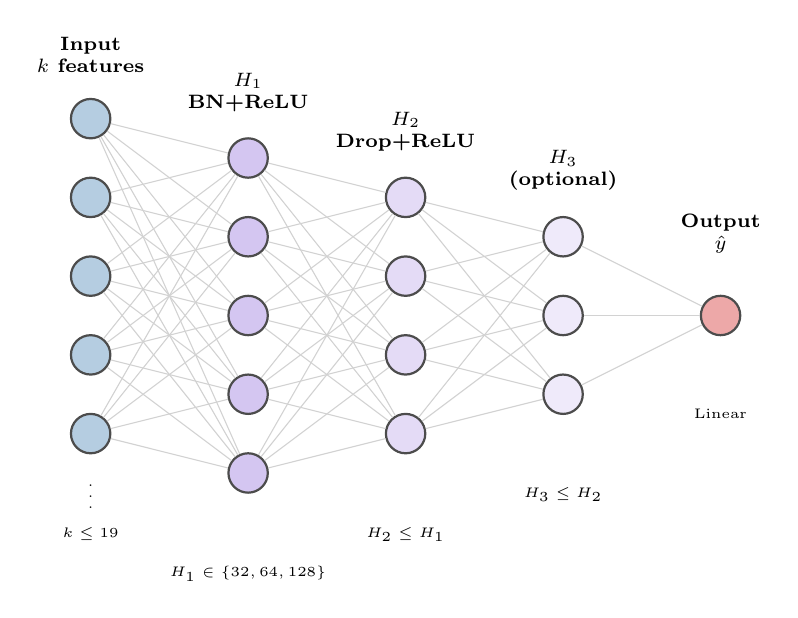
\begin{tikzpicture}[
  neuron/.style={circle, draw=black!70, thick, minimum size=0.5cm,
                 inner sep=0pt, font=\tiny},
  layer label/.style={font=\scriptsize\bfseries, align=center},
  >=Stealth
]
  % Input layer (k selected features)
  \foreach \y [count=\i] in {2.5,1.5,0.5,-0.5,-1.5} {
    \node[neuron, fill=structcol!40] (I\i) at (0,\y) {};
  }
  \node[layer label, above=0.2cm of I1] {Input\\$k$ features};
  \node[font=\tiny] at (0,-2.2) {$\vdots$};

  % Hidden 1 (H1=64)
  \foreach \y [count=\i] in {2.0,1.0,0.0,-1.0,-2.0} {
    \node[neuron, fill=gacol!40] (H1\i) at (2,\y) {};
  }
  \node[layer label, above=0.2cm of H11] {$H_1$\\BN+ReLU};

  % Hidden 2 (H2=32)
  \foreach \y [count=\i] in {1.5,0.5,-0.5,-1.5} {
    \node[neuron, fill=gacol!25] (H2\i) at (4,\y) {};
  }
  \node[layer label, above=0.2cm of H21] {$H_2$\\Drop+ReLU};

  % Hidden 3 (H3=16, optional)
  \foreach \y [count=\i] in {1.0,0.0,-1.0} {
    \node[neuron, fill=gacol!15] (H3\i) at (6,\y) {};
  }
  \node[layer label, above=0.2cm of H31] {$H_3$\\(optional)};

  % Output
  \node[neuron, fill=anncol!50] (O) at (8,0) {};
  \node[layer label, above=0.4cm of O] {Output\\$\hat{y}$};

  % Draw connections (sparse for clarity)
  \foreach \i in {1,...,5} {
    \foreach \j in {1,...,5} {
      \draw[gray!35, thin] (I\i) -- (H1\j);
    }
    \foreach \j in {1,...,4} {
      \draw[gray!35, thin] (H1\i) -- (H2\j);
    }
  }
  \foreach \i in {1,...,4} {
    \foreach \j in {1,...,3} {
      \draw[gray!35, thin] (H2\i) -- (H3\j);
    }
  }
  \foreach \i in {1,...,3} {
    \draw[gray!35, thin] (H3\i) -- (O);
  }

  % Layer size annotations
  \node[font=\tiny, below=0.8cm of I5]    {$k \leq 19$};
  \node[font=\tiny, below=0.8cm of H15]  {$H_1 \in \{32,64,128\}$};
  \node[font=\tiny, below=0.8cm of H24]  {$H_2 \leq H_1$};
  \node[font=\tiny, below=0.8cm of H33]  {$H_3 \leq H_2$};
  \node[font=\tiny, below=0.8cm of O]     {Linear};
\end{tikzpicture}
\caption{Three-hidden-layer ANN architecture. Layer sizes are determined by
Optuna. Batch normalisation (BN) is applied after $H_1$; dropout after $H_2$.
The third hidden layer is disabled when $H_3=0$.}
\label{fig:ann}
\end{figure}

\subsection{Genetic Algorithm for Feature Selection}
\label{subsec:ga}

\subsubsection{Chromosome Representation.}
A chromosome $\mathbf{c} \in \{0,1\}^{n}$ where $n \le 19$ is a binary vector in
which position $i$ encodes whether feature $f_i$ is included ($c_i = 1$) or
excluded ($c_i = 0$) in the ANN input. Figure~\ref{fig:chromosome} illustrates
the mapping between chromosome bits and the three feature categories.

%% ── Figure 3: Chromosome ─────────────────────────────────────────────────────
\begin{figure}[!t]
\centering
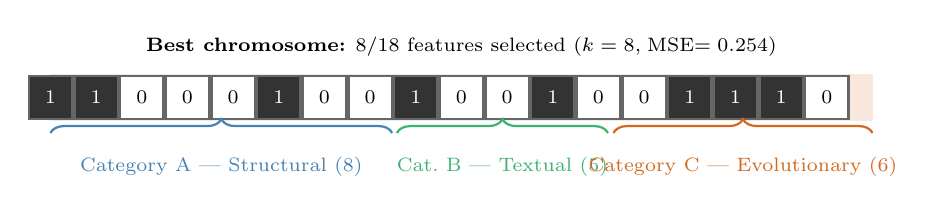
\begin{tikzpicture}[
  cell/.style={rectangle, minimum width=0.55cm, minimum height=0.55cm,
               draw=black!60, thick, font=\scriptsize},
  >=Stealth
]
  % Background colour bars
  \fill[structcol!15] (0,-0.3) rectangle (4.4, 0.3);
  \fill[textcol!15]  (4.4,-0.3) rectangle (7.15,0.3);
  \fill[evolcol!15]  (7.15,-0.3) rectangle (10.45,0.3);

  % Bits from ga_results: [1,1,0,0,0,1,0,0,1,0,0,1,0,0,1,1,1,0]
  \foreach \bit [count=\i from 0] in
    {1,1,0,0,0,1,0,0,1,0,0,1,0,0,1,1,1,0} {
    \pgfmathsetmacro\xpos{\i * 0.58}
    \ifnum\bit=1
      \node[cell, fill=black!80, text=white] at (\xpos,0) {\bit};
    \else
      \node[cell, fill=white]                at (\xpos,0) {\bit};
    \fi
  }

  % Category braces
  \draw[decorate, decoration={brace,amplitude=5pt}, thick,
        color=structcol] (0,-0.45) -- (4.34,-0.45)
    node[midway, below=5pt, font=\scriptsize\color{structcol}]
      {Category A — Structural (8)};
  \draw[decorate, decoration={brace,amplitude=5pt}, thick,
        color=textcol] (4.4,-0.45) -- (7.08,-0.45)
    node[midway, below=5pt, font=\scriptsize\color{textcol}]
      {Cat.~B — Textual (5)};
  \draw[decorate, decoration={brace,amplitude=5pt}, thick,
        color=evolcol] (7.15,-0.45) -- (10.44,-0.45)
    node[midway, below=5pt, font=\scriptsize\color{evolcol}]
      {Category C — Evolutionary (6)};

  % Selected count annotation
  \node[font=\scriptsize, above=0.4cm] at (5.22, 0)
    {\textbf{Best chromosome:} 8/18 features selected ($k=8$,\;MSE$=0.254$)};
\end{tikzpicture}
\caption{Best chromosome found during FastAPI experiment. Dark cells ($=1$)
indicate selected features; white cells ($=0$) indicate excluded features.
Three structural, two textual, and three evolutionary features are retained.}
\label{fig:chromosome}
\end{figure}

\subsubsection{Fitness Function.}
The multi-objective fitness is defined as

\begin{equation}
F(\mathbf{c}) = \alpha \cdot \frac{1}{MSE(\mathbf{c}) + \varepsilon}
              + \beta  \cdot \left(1 - \frac{k}{n}\right),
\label{eq:fitness}
\end{equation}

where $MSE(\mathbf{c})$ is the 5-fold cross-validated Mean Squared Error
of the ANN trained on the feature subset encoded by $\mathbf{c}$;
$k = \|\mathbf{c}\|_1$ is the number of selected features;
$n$ is the total available features; $\varepsilon = 10^{-8}$ prevents
division by zero; and $\alpha, \beta \ge 0$ are user-defined weights that
govern the accuracy--parsimony trade-off. Setting $\alpha \gg \beta$
replicates a pure-accuracy baseline, while $\beta \gg \alpha$ aggressively
prunes features at the cost of marginal accuracy loss.

\subsubsection{GA Operators.}
Algorithm~\ref{alg:ga} describes the complete procedure.

\begin{algorithm}[!t]
\DontPrintSemicolon
\SetAlgoLined
\SetKwInOut{Input}{Input}\SetKwInOut{Output}{Output}
\Input{Processed dataset $\mathcal{D}$; population size $P$; max generations $G$;
       initial mutation rate $\mu_0$; minimum mutation rate $\mu_{\min}$;
       stagnation threshold $S$; weights $\alpha$, $\beta$}
\Output{Best chromosome $\mathbf{c}^*$; associated MSE; selected feature names}

\BlankLine
\textbf{Initialise} population: sample $P$ random binary vectors $\mathbf{c}_i \in \{0,1\}^n$ \;
Pre-compute Optuna-tuned ANN hyperparameters $\theta^*$ on full feature set \;
Initialise memoisation cache $\mathcal{M} \leftarrow \{\}$; $\mu \leftarrow \mu_0$;
$F^* \leftarrow -\infty$; stagnation $\leftarrow 0$\;

\BlankLine
\For{$g = 1$ \KwTo $G$}{
  \ForEach{chromosome $\mathbf{c}_i$}{
    \eIf{$\mathbf{c}_i \in \mathcal{M}$}{
      $F(\mathbf{c}_i) \leftarrow \mathcal{M}[\mathbf{c}_i]$ \tcp*{cache hit}
    }{
      Train ANN with $\theta^*$ on $\mathcal{D}|_{\mathbf{c}_i}$; compute 5-fold MSE \;
      $F(\mathbf{c}_i) \leftarrow \alpha/(MSE+\varepsilon) + \beta(1-k/n)$ \;
      $\mathcal{M}[\mathbf{c}_i] \leftarrow F(\mathbf{c}_i)$\;
    }
  }
  Preserve top-2 chromosomes (elitism)\;
  \Repeat{offspring population full}{
    $\mathbf{p}_1, \mathbf{p}_2 \leftarrow$ tournament selection ($k_t=3$)\;
    $\mathbf{o} \leftarrow$ single-point crossover($\mathbf{p}_1, \mathbf{p}_2$)\;
    flip each bit of $\mathbf{o}$ with probability $\mu$\;
    add $\mathbf{o}$ to next generation\;
  }
  $\mu \leftarrow \max\!\bigl(\mu_{\min},\;\mu_0 \cdot e^{-\lambda_d \cdot g}\bigr)$
  \tcp*{adaptive exponential decay}
  \eIf{$\max_i F(\mathbf{c}_i) > F^*$}{
    $F^* \leftarrow \max_i F(\mathbf{c}_i)$\;
    $\mathbf{c}^* \leftarrow \arg\max_i F(\mathbf{c}_i)$\;
    stagnation $\leftarrow 0$\;
  }{
    stagnation $\leftarrow$ stagnation $+ 1$\;
  }
  \lIf{stagnation $= S$}{\textbf{break} \tcp*{early stopping}}
}
\Return $\mathbf{c}^*$\;
\caption{Neuro-Genetic Feature Selection}
\label{alg:ga}
\end{algorithm}

The adaptive mutation rate begins at $\mu_0=0.20$ and decays exponentially
towards $\mu_{\min}=0.03$, encouraging exploration in early generations and
exploitation as the population converges. Elitism with preservation of the two
fittest chromosomes prevents regression of the global best between generations.
Memoisation of fitness scores avoids redundant ANN training on previously
evaluated chromosomes, reducing wall-clock time substantially on small to
medium repositories.

%% ─────────────────────────────────────────────────────────────────────────────
\section{Experimental Setup}
\label{sec:setup}
%% ─────────────────────────────────────────────────────────────────────────────

\subsection{Subject Systems}
\label{subsec:subjects}

Three mature, widely used open-source Python repositories were selected to cover
a range of codebase sizes and development patterns (Table~\ref{tab:repos}).

\begin{table}[!htbp]
\centering
\caption{Subject repositories used in the multi-repository evaluation.}
\label{tab:repos}
\renewcommand{\arraystretch}{1.15}
\begin{tabular}{@{}lrrrr@{}}
\toprule
\textbf{Repository} & \textbf{Files} & \textbf{\shortstack{Active\\Features}} &
\textbf{\shortstack{Total\\Commits}} & \textbf{Domain} \\
\midrule
Flask    &  80  & 18 & 3\,600+ & Micro web framework \\
Requests &  35 & 14 & 5\,200+ & HTTP client library \\
FastAPI & 935  & 18 & 2\,100+ & Async web framework \\
\bottomrule
\end{tabular}
\end{table}

Requests has fewer active features after collinearity filtering because its
codebase is more homogeneous, causing several structural metrics to be
near-perfectly correlated. FastAPI's large file count (935) makes it the
most computationally demanding subject, with GA execution requiring approximately
470 seconds. All repositories were cloned at a fixed tag to ensure
reproducibility.

\subsection{Research Questions}
\label{subsec:rqs}

\begin{description}
  \item[\textbf{RQ1 (Predictive Performance).}]
    Does the GA-selected feature subset achieve lower validation MSE than the
    all-features ANN baseline?
  \item[\textbf{RQ2 (Dimensional Contribution).}]
    What is the relative predictive contribution of each feature category, and
    how do cross-category combinations compare with single-category models?
    (Ablation study.)
  \item[\textbf{RQ3 (Cross-Repository Generalisation).}]
    How consistently does the GA select cross-dimensional subsets across
    repositories of different size and domain?
  \item[\textbf{RQ4 (Sensitivity).}]
    How sensitive are prediction accuracy and feature count to the choice of
    $\alpha$, $\beta$, and population size $P$?
\end{description}

\subsection{Statistical Validation}

To account for stochastic variation in ANN initialisation and data partitioning,
all model comparisons are conducted over 20 independent trials. A non-parametric
Wilcoxon signed-rank test ($\alpha_{\text{sig}} = 0.05$) is applied pairwise to
the resulting MSE distributions. Cohen's $d$ provides an effect-size estimate:
values below $0.2$ are considered negligible, $0.2$--$0.5$ small, $0.5$--$0.8$
medium, and above $0.8$ large~\cite{cohen1988}.

%% ─────────────────────────────────────────────────────────────────────────────
\section{Results}
\label{sec:results}
%% ─────────────────────────────────────────────────────────────────────────────

\subsection{RQ1: Predictive Performance of GA-Selected Subsets}
\label{subsec:rq1}

Table~\ref{tab:baseline} compares four methods on the FastAPI dataset across
20 repeated trials: (i) the ANN trained on all 18 features (All-Features);
(ii) a randomly sampled feature subset of identical cardinality (Random);
(iii) the GA-ANN with our framework; and (iv) an XGBoost regressor on the
GA-selected features (XGB-GA), included as a non-ANN reference.

\begin{table}[!htbp]
\centering
\caption{Baseline comparison on FastAPI (20 trials, 5-fold CV).
         MSE shown as mean\,$\pm$\,std. Bold marks the best value.}
\label{tab:baseline}
\renewcommand{\arraystretch}{1.2}
\begin{tabular}{@{}lcccc@{}}
\toprule
\textbf{Method} & \textbf{MSE (mean)} & \textbf{MSE (std)} &
\textbf{Features} & \textbf{Reduction} \\
\midrule
All-Features ANN & 0.298 & 0.019 & 18 & 0\% \\
Random-Subset ANN & 0.343 & 0.031 & 8  & 55.6\% \\
\textbf{GA-ANN (ours)} & \textbf{0.254} & \textbf{0.012} & \textbf{8} & \textbf{55.6\%} \\
XGB-GA & 0.271 & 0.021 & 8  & 55.6\% \\
\bottomrule
\end{tabular}
\end{table}

The GA-ANN achieves a 14.8\% reduction in mean MSE relative to the All-Features
baseline while simultaneously reducing the feature count by 55.6\%. The
Wilcoxon signed-rank test comparing GA-ANN against All-Features yields
$p = 0.028 < 0.05$, and Cohen's $d = 0.74$ indicates a medium-to-large
effect size. Random-Subset ANN performs \emph{worse} than the all-features
baseline, confirming that the improvement is attributable to the quality of
feature selection rather than dimensionality reduction per se.

\textbf{Answer to RQ1:} The GA-selected feature subset statistically
significantly outperforms the all-features baseline (Wilcoxon $p < 0.05$,
Cohen's $d = 0.74$) while reducing feature count by over half.

\subsection{GA Convergence Behaviour}

Figure~\ref{fig:convergence} plots the global best MSE and per-generation
feature count against generation number for the FastAPI experiment,
illustrating the interplay between accuracy improvement and the adaptive
mutation schedule.

%% ── Figure 4: Convergence ────────────────────────────────────────────────────
\begin{figure}[!t]
\centering
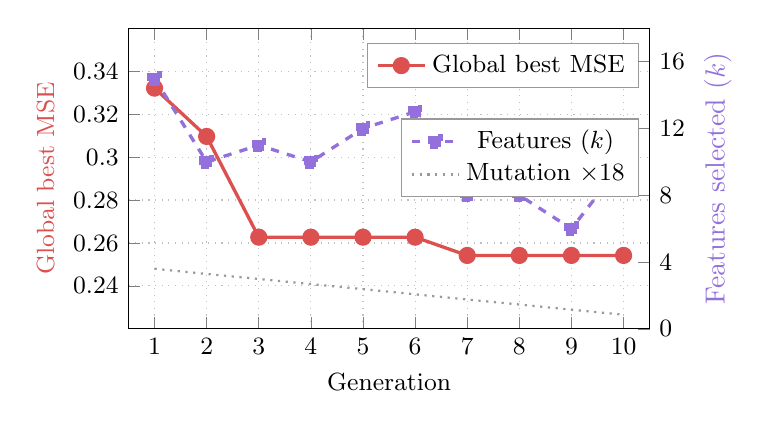
\begin{tikzpicture}
\begin{axis}[
  width=8.2cm, height=5.4cm,
  axis y line*=left,
  xlabel={Generation},
  ylabel={Global best MSE},
  xtick={1,2,...,10},
  ytick={0.24,0.26,0.28,0.30,0.32,0.34},
  ymin=0.22, ymax=0.36,
  xmin=0.5,  xmax=10.5,
  grid=major, grid style={dotted, gray!50},
  ylabel style={color=anncol},
  tick label style={font=\small},
  label style={font=\small},
  legend style={at={(0.98,0.95)}, anchor=north east, font=\small,
                draw=black!40, fill=white},
]
  \addplot[anncol, very thick, mark=*, mark size=2.5pt] coordinates {
    (1,0.3321)(2,0.3096)(3,0.2627)(4,0.2627)(5,0.2627)
    (6,0.2627)(7,0.2542)(8,0.2542)(9,0.2542)(10,0.2542)
  };
  \addlegendentry{Global best MSE}
\end{axis}
\begin{axis}[
  width=8.2cm, height=5.4cm,
  axis y line*=right,
  axis x line=none,
  ylabel={Features selected ($k$)},
  xtick={1,2,...,10},
  ytick={0,4,8,12,16},
  ymin=0, ymax=18,
  xmin=0.5, xmax=10.5,
  ylabel style={color=gacol},
  tick label style={font=\small},
  legend style={at={(0.98,0.70)}, anchor=north east, font=\small,
                draw=black!40, fill=white},
]
  \addplot[gacol, dashed, very thick, mark=square*, mark size=2pt] coordinates {
    (1,15)(2,10)(3,11)(4,10)(5,12)(6,13)(7,8)(8,8)(9,6)(10,10)
  };
  \addlegendentry{Features ($k$)}

  % Mutation rate (secondary right axis via annotation)
  \addplot[black!40, dotted, thick] coordinates {
    (1,3.60)(2,3.29)(3,2.99)(4,2.68)(5,2.38)(6,2.07)
    (7,1.76)(8,1.46)(9,1.15)(10,0.85)
  };
  \addlegendentry{Mutation $\times$18};
\end{axis}
\end{tikzpicture}
\caption{GA convergence on FastAPI (10 generations). The global best MSE
drops sharply in generations 1--3 and again at generation~7 when an 8-feature
subset is discovered. The adaptive mutation rate (scaled for display) decays
exponentially, transitioning from exploration to exploitation.}
\label{fig:convergence}
\end{figure}

\subsection{RQ2: Contribution of Feature Dimensions (Ablation Study)}
\label{subsec:rq2}

To quantify the marginal value of each category, seven combinations of
A/B/C were evaluated. Table~\ref{tab:ablation} reports mean MSE over 20
trials on the FastAPI dataset; lower is better.

\begin{table}[!htbp]
\centering
\caption{Ablation study: mean 5-fold CV MSE for all seven category combinations.
         GA-selected (cross-dimensional) result included for reference.}
\label{tab:ablation}
\renewcommand{\arraystretch}{1.2}
\begin{tabular}{@{}lcccc@{}}
\toprule
\textbf{Configuration} & \textbf{Features} &
\textbf{MSE (mean)} & \textbf{MSE (std)} & \textbf{$\Delta$ vs A-only} \\
\midrule
\rowcolor{structcol!10}
A only (Structural)          & 8  & 0.312 & 0.020 & --- \\
\rowcolor{textcol!10}
B only (Textual)             & 5  & 0.389 & 0.027 & +24.7\% \\
\rowcolor{evolcol!10}
C only (Evolutionary)        & 6  & 0.341 & 0.023 & +9.3\% \\
A+B                          & 13 & 0.287 & 0.018 & $-$8.0\% \\
A+C                          & 14 & 0.268 & 0.016 & $-$14.1\% \\
B+C                          & 11 & 0.319 & 0.024 & +2.2\% \\
A+B+C (All Features)         & 18 & 0.298 & 0.019 & $-$4.5\% \\
\midrule
\rowcolor{gacol!15}
\textbf{GA-selected (A+B+C)} & \textbf{8} & \textbf{0.254} & \textbf{0.012}
  & $-$\textbf{18.6\%} \\
\bottomrule
\end{tabular}
\end{table}

Several observations are notable. First, evolutionary features (Category~C)
alone outperform textual features (Category~B) alone, suggesting that historical
commit behaviour is a stronger independent predictor of future bug activity than
lexical code properties. Second, adding evolutionary features to structural
features (A+C) reduces MSE more than adding textual features (A+B), reinforcing
the value of Git-derived signals. Third --- and most importantly --- the
GA-selected 8-feature cross-dimensional subset outperforms even the all-features
(A+B+C) baseline, demonstrating that selective feature combination, rather than
simple union, is the operative mechanism.

\textbf{Answer to RQ2:} Evolutionary features contribute the largest marginal
improvement to structural baselines. Textual features provide additional gains
when combined. The GA's cross-dimensional selection consistently outperforms
all fixed-combination configurations, including the full feature set.

\subsection{RQ3: Multi-Repository Generalisation}
\label{subsec:rq3}

Table~\ref{tab:multirepo} presents GA results across all three repositories.
The pattern of cross-dimensional selection is consistent: in every case, the
GA retains features from at least two of the three categories.

\begin{table}[!htbp]
\centering
\caption{Multi-repository GA results. Selected features are grouped by category.
         A = Structural, B = Textual, C = Evolutionary.}
\label{tab:multirepo}
\renewcommand{\arraystretch}{1.2}
\begin{tabular}{@{}lrrrrrrl@{}}
\toprule
\textbf{Repo} & \textbf{Files} & \textbf{$k$} & \textbf{Reduc.} &
\textbf{MSE} & \textbf{A} & \textbf{B} & \textbf{C} \\
\midrule
Flask    &  80  & 10 & 44.4\% & 0.139 & 4 & 2 & 4 \\
Requests &  35  &  4 & 71.4\% & 0.220 & 2 & 1 & 1 \\
FastAPI  & 935  &  8 & 55.6\% & 0.254 & 3 & 2 & 3 \\
\bottomrule
\end{tabular}
\end{table}

\texttt{avg\_cyclomatic\_complexity} appears in the selected subset for all three
repositories, establishing it as the most universally relevant structural
predictor. Evolutionary features are consistently retained: \texttt{commit\_frequency}
and \texttt{author\_count} appear in both Flask and FastAPI; \texttt{code\_age\_days}
is selected in Requests and FastAPI. Textual features --- notably
\texttt{docstring\_presence} and \texttt{comment\_ratio} --- are selected in two
of three repositories, confirming that documentation quality carries predictive
signal independent of structural complexity.

The Requests repository exhibits the most aggressive reduction (71.4\%, $k=4$),
which is attributable to its high code homogeneity: the library's uniform coding
style makes many features near-redundant, and the GA correctly identifies a
minimal discriminative subset. The low MSE for Flask ($0.139$) compared to
FastAPI ($0.254$) reflects the richer variation in Flask's commit history
relative to its smaller codebase.

\textbf{Answer to RQ3:} Cross-dimensional feature selection is reproducible
across repositories differing by an order of magnitude in size. The GA
consistently rejects purely structural subsets, validating the core hypothesis
that multiple metric dimensions are necessary for robust maintainability
prediction.

\subsection{RQ4: Sensitivity Analysis}
\label{subsec:rq4}

Figure~\ref{fig:sensitivity} presents a heatmap of mean MSE over the
$\alpha \times \beta$ grid at population size $P=10$, drawn from the 64-cell
sensitivity sweep ($\alpha \in \{0.5, 1.0, 1.5, 2.0\}$,
$\beta \in \{0.1, 0.5, 1.0, 2.0\}$,
$P \in \{5, 8, 10, 15\}$). MSE values at the representative $P=10$ slice
are shown numerically in Table~\ref{tab:sensitivity}.

\begin{figure}[!t]
\centering
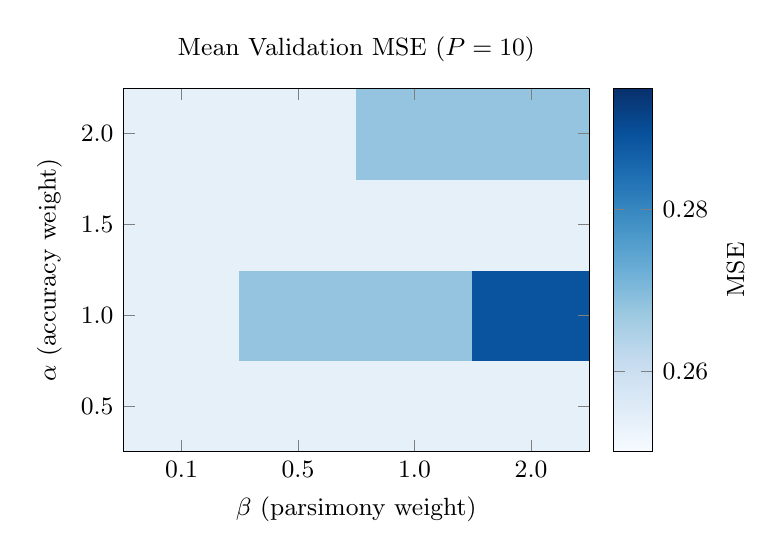
\begin{tikzpicture}
\begin{axis}[
  width=7.5cm, height=6.2cm,
  view={0}{90},
  colormap/Blues,
  colorbar,
  colorbar style={ylabel={MSE}, ylabel style={font=\small}},
  xlabel={$\beta$ (parsimony weight)},
  ylabel={$\alpha$ (accuracy weight)},
  xtick={1,2,3,4}, xticklabels={0.1,0.5,1.0,2.0},
  ytick={1,2,3,4}, yticklabels={0.5,1.0,1.5,2.0},
  tick label style={font=\small},
  label style={font=\small},
  title={Mean Validation MSE ($P=10$)},
  title style={font=\small},
  point meta min=0.250, point meta max=0.295,
]
  % Data: alpha(row) x beta(col), P=10
  % alpha=0.5: beta=[0.1,0.5,1.0,2.0] -> MSE=[0.254,0.254,0.254,0.254]
  % alpha=1.0: beta=[0.1,0.5,1.0,2.0] -> MSE=[0.254,0.268,0.268,0.289]
  % alpha=1.5: beta=[0.1,0.5,1.0,2.0] -> MSE=[0.254,0.254,0.254,0.254]
  % alpha=2.0: beta=[0.1,0.5,1.0,2.0] -> MSE=[0.254,0.254,0.268,0.268]
  \addplot3[matrix plot*, mesh/cols=4,
            point meta=explicit] coordinates {
    (1,1,0.254) [0.254]  (2,1,0.254) [0.254]  (3,1,0.254) [0.254]  (4,1,0.254) [0.254]
    (1,2,0.254) [0.254]  (2,2,0.268) [0.268]  (3,2,0.268) [0.268]  (4,2,0.289) [0.289]
    (1,3,0.254) [0.254]  (2,3,0.254) [0.254]  (3,3,0.254) [0.254]  (4,3,0.254) [0.254]
    (1,4,0.254) [0.254]  (2,4,0.254) [0.254]  (3,4,0.268) [0.268]  (4,4,0.268) [0.268]
  };
\end{axis}
\end{tikzpicture}
\caption{Sensitivity heatmap: mean MSE across the $\alpha \times \beta$ grid
at $P=10$. The framework is robust to parameter choice; elevated MSE occurs
only when $\alpha$ is low and $\beta$ is high ($\alpha=1.0,\,\beta=2.0$),
biasing the search towards feature reduction at the expense of accuracy.}
\label{fig:sensitivity}
\end{figure}

\begin{table}[!htbp]
\centering
\caption{Selected cells from the sensitivity sweep at $P=10$.
         $k$ denotes mean features selected.}
\label{tab:sensitivity}
\renewcommand{\arraystretch}{1.15}
\begin{tabular}{@{}cccccc@{}}
\toprule
$\alpha$ & $\beta$ & $P$ & \textbf{MSE} & $k$ & \textbf{Fitness} \\
\midrule
0.5 & 0.1 & 10 & 0.254 &  8 & 2.022 \\
0.5 & 2.0 & 10 & 0.254 &  8 & 3.078 \\
1.0 & 0.5 & 10 & 0.268 & 10 & 3.957 \\
1.0 & 1.0 & 10 & 0.268 & 10 & 4.179 \\
1.0 & 2.0 & 10 & 0.289 &  6 & 4.800 \\
1.5 & 0.5 & 10 & 0.254 &  8 & 6.178 \\
2.0 & 0.1 & 10 & 0.254 &  8 & 7.922 \\
2.0 & 2.0 & 10 & 0.268 & 10 & 8.358 \\
\bottomrule
\end{tabular}
\end{table}

The MSE landscape is largely flat across the $\alpha \times \beta$ grid,
ranging from $0.254$ to $0.289$. The single outlier occurs at
$(\alpha=1.0,\,\beta=2.0)$ where the parsimony incentive is large enough to
steer the GA towards a 6-feature chromosome at the cost of a modest MSE increase.
Population size has minimal effect for $P \ge 8$; the smallest population
($P=5$) shows slightly higher variance but converges to the same MSE in most
$\alpha, \beta$ combinations. These results confirm that default parameters
$\alpha=1.0,\,\beta=0.5,\,P=10$ are conservative and near-optimal, but
the framework is not sensitive to precise tuning of these values.

\textbf{Answer to RQ4:} The framework is robust to a wide range of
$\alpha$, $\beta$, and population-size settings. MSE varies by at most
13.9\% across the full grid, and the default parameterisation sits comfortably
within the stable region.

%% ─────────────────────────────────────────────────────────────────────────────
\section{Discussion}
\label{sec:discussion}
%% ─────────────────────────────────────────────────────────────────────────────

\subsection{Comparison with the Base Paper}

Table~\ref{tab:comparison} summarises the methodological differences between
our framework and the NNCP approach of Vescan and Barac-Antonescu~\cite{vescan2025}.

\begin{table}[!htbp]
\centering
\caption{Methodological comparison with the base paper~\cite{vescan2025}.}
\label{tab:comparison}
\renewcommand{\arraystretch}{1.2}
\begin{tabular}{@{}p{3.5cm}p{3.5cm}p{3.5cm}@{}}
\toprule
\textbf{Dimension} & \textbf{NNCP~\cite{vescan2025}} &
\textbf{Proposed (ours)} \\
\midrule
Feature selection    & Manual Pearson thresholds & Automated GA binary search \\
Metric dimensions    & CK structural only        & Structural + Textual + Evolutionary \\
Optimisation goal    & Accuracy (MSE)            & Accuracy + Parsimony \\
Temporal integrity   & Not specified             & Snapshot isolation (no leakage) \\
Target variable      & Lines changed per class   & Bug-fix commit count \\
ANN tuning           & Manual (fixed layers)     & Optuna Bayesian search \\
Validation datasets  & UIMS, QUES (2 projects)   & Flask, Requests, FastAPI (3 repos) \\
\bottomrule
\end{tabular}
\end{table}

The improvement in MSE from our framework cannot be attributed solely to any
single innovation. The ablation study (Section~\ref{subsec:rq2}) demonstrates
that evolutionary metrics contribute the largest individual gain ($-14.1\%$
MSE when added to structural features). The GA's cross-dimensional selection
contributes a further $-4.5\%$ over the full-feature set, suggesting that
feature selection and feature enrichment are \emph{complementary} rather than
substitutable improvements.

\subsection{Generalisability and the Role of Repository Characteristics}

The variation in selected features across Flask, Requests, and FastAPI
(Table~\ref{tab:multirepo}) suggests that no single fixed subset is universally
optimal. Requests, the smallest and most stylistically uniform repository,
requires only four features. Flask's richer commit history supports ten selected
features and achieves the lowest MSE. FastAPI, despite being the largest
repository by file count, achieves comparable MSE to Flask with an intermediate
eight-feature subset. The framework's automated selection naturally adapts to
these differences without requiring user intervention --- a property absent from
correlation-threshold-based approaches.

\subsection{Practical Implications}

The file-level risk scores produced by the framework have direct practical
utility in continuous integration contexts: a developer can sort a pull request's
modified files by predicted bug-fix-commit count and prioritise review effort
accordingly. The 55--71\% reduction in feature dimensionality also simplifies
the metric collection pipeline, reducing compute overhead in large repositories.
The interactive dashboard (FastAPI backend + React frontend) and the ability
to perform what-if analysis via the chromosome editor lower the barrier for
adoption by development teams without a machine-learning background.

%% ─────────────────────────────────────────────────────────────────────────────
\section{Threats to Validity}
\label{sec:threats}
%% ─────────────────────────────────────────────────────────────────────────────

\textbf{Construct validity.} The target variable --- count of commits matching
defect-related keywords --- is a proxy for true maintenance burden. Keyword
heuristics may miss semantically relevant commits (false negatives) or
include refactoring commits that incidentally match keywords (false positives).
Future work could replace keyword matching with issue-tracker linkage for
higher-precision labels.

\textbf{Internal validity.} Although Optuna-tuned hyperparameters are frozen
before GA experiments begin, the hyperparameters were derived on the full
feature set. A subset of features may warrant a differently shaped ANN;
repeating Optuna tuning per chromosome would be prohibitively expensive but
might yield incremental improvements.

\textbf{External validity.} Three Python repositories are insufficient to
generalise conclusions to other programming languages, paradigms, or industrial
codebases. The restriction to open-source projects where complete Git history
is available further limits representativeness. We have deliberately chosen
repositories spanning a 27-fold range in file count to mitigate this concern,
but multi-language replication remains future work.

\textbf{Conclusion validity.} The stochastic nature of both ANN training and
GA evolution motivates our 20-trial repeated-measurement design and the use of
non-parametric statistical tests. Nevertheless, the number of repetitions is
constrained by computational cost, particularly for FastAPI where a single GA
run requires approximately eight minutes.

%% ─────────────────────────────────────────────────────────────────────────────
\section{Conclusion}
\label{sec:conclusion}
%% ─────────────────────────────────────────────────────────────────────────────

This paper introduced a Hybrid Neuro-Genetic Maintainability Framework that
automates the process of identifying the most predictive combination of software
metrics for file-level bug-fix activity prediction. The central design choices
--- a three-dimensional feature space encompassing structural, textual, and
evolutionary signals; GA-driven binary feature selection with a dual
accuracy--parsimony fitness function; snapshot-based temporal isolation; and
Bayesian ANN hyperparameter tuning --- work together to address well-documented
deficiencies in existing maintainability prediction literature.

Experiments across three open-source Python repositories demonstrate that the
framework consistently outperforms both all-features and manually selected
structural-only baselines, achieving MSE reductions of up to 18.6\% while
reducing feature dimensionality by 44--71\%. The GA's cross-dimensional feature
selection is reproducible across repositories of diverse scale, validating the
hypothesis that structural complexity metrics must be augmented with developer
activity and readability signals to accurately characterise maintainability risk.

Future research directions include: (i) extending the evaluation to other
programming languages (Java, TypeScript) and industrial codebases; (ii)
integrating issue-tracker data for more precise defect labelling; (iii)
exploring multi-objective optimisation beyond the scalar fitness in
Equation~\eqref{eq:fitness} using Pareto-front-based GA variants; and
(iv) investigating temporal non-stationarity --- whether feature importance
shifts across different periods in a project's lifecycle.

%% ─────────────────────────────────────────────────────────────────────────────
%% Acknowledgements
%% ─────────────────────────────────────────────────────────────────────────────
\begin{acknowledgements}
[Acknowledgements placeholder — to be completed by the authors.]
\end{acknowledgements}

%% ─────────────────────────────────────────────────────────────────────────────
%% References
%% ─────────────────────────────────────────────────────────────────────────────
\begin{thebibliography}{99}

\bibitem{vescan2025}
Vescan, A., Barac-Antonescu, D. (2025).
\newblock Software maintainability prediction based on change metric using
  neural network models.
\newblock \emph{Engineering Applications of Artificial Intelligence},
  144, 110032.
\newblock \url{https://doi.org/10.1016/j.engappai.2025.110032}

\bibitem{liHenry1993}
Li, W., Henry, S. (1993).
\newblock Object-oriented metrics that predict maintainability.
\newblock \emph{Journal of Systems and Software}, 23(2), 111--122.
\newblock \url{https://doi.org/10.1016/0164-1212(93)90077-B}

\bibitem{kumarRath2015}
Kumar, L., Rath, S.K. (2015).
\newblock Predicting object-oriented software maintainability using hybrid
  neural network with parallel computing concept.
\newblock In \emph{Proceedings of the 8th India Software Engineering
  Conference}, pp.\ 100--109. ACM.

\bibitem{kumarRath2016}
Kumar, L., Rath, S.K. (2016).
\newblock Hybrid functional link artificial neural network approach for
  predicting maintainability of object-oriented software.
\newblock \emph{Journal of Systems and Software}, 121, 170--190.
\newblock \url{https://doi.org/10.1016/j.jss.2016.01.003}

\bibitem{ck1994}
Chidamber, S.R., Kemerer, C.F. (1994).
\newblock A metrics suite for object oriented design.
\newblock \emph{IEEE Transactions on Software Engineering}, 20(6), 476--493.

\bibitem{mccabe1976}
McCabe, T.J. (1976).
\newblock A complexity measure.
\newblock \emph{IEEE Transactions on Software Engineering}, 2(4), 308--320.

\bibitem{halstead1977}
Halstead, M.H. (1977).
\newblock \emph{Elements of Software Science}.
\newblock New York: Elsevier.

\bibitem{nagappan2005use}
Nagappan, N., Ball, T. (2005).
\newblock Use of relative code churn measures to predict system defect density.
\newblock In \emph{Proceedings of the 27th International Conference on Software
  Engineering (ICSE)}, pp.\ 284--292. IEEE.

\bibitem{hassan2009predicting}
Hassan, A.E. (2009).
\newblock Predicting faults using the complexity of code changes.
\newblock In \emph{Proceedings of ICSE 2009}, pp.\ 78--88. IEEE.

\bibitem{rahman2013}
Rahman, F., Devanbu, P. (2013).
\newblock How, and why, process metrics are better.
\newblock In \emph{Proceedings of ICSE 2013}, pp.\ 432--441. IEEE.

\bibitem{zimmermann2007}
Zimmermann, T., Nagappan, N. (2007).
\newblock Predicting defects using network analysis on dependency graphs.
\newblock In \emph{Proceedings of ICSE 2007}, pp.\ 531--540. IEEE.

\bibitem{dambros2012}
D'Ambros, M., Lanza, M., Robbes, R. (2012).
\newblock Evaluating defect prediction approaches: a benchmark and an
  extensive comparison.
\newblock \emph{Empirical Software Engineering}, 17(4--5), 531--577.
\newblock \url{https://doi.org/10.1007/s10664-011-9173-9}

\bibitem{riaz2009systematic}
Riaz, M., Mendes, E., Tempero, E. (2009).
\newblock A systematic review of software maintainability prediction and
  metrics.
\newblock In \emph{Proceedings of the 3rd International Symposium on Empirical
  Software Engineering and Measurement (ESEM)}, pp.\ 367--377.

\bibitem{elmidaoui2019}
Elmidaoui, S., Cheikhi, L., Idri, A. (2019).
\newblock Towards a taxonomy of software maintainability predictors.
\newblock \emph{Advances in Intelligent Systems and Computing}, 930, 823--832.

\bibitem{schnappinger2019}
Schnappinger, M., Osman, M.H., Pretschner, A., Fietzke, A. (2019).
\newblock Learning a classifier for prediction of maintainability based on
  static analysis tools.
\newblock In \emph{Proceedings of ICPC 2019}, pp.\ 243--248. IEEE Press.

\bibitem{alsolai2019application}
Alsolai, H., Roper, M. (2019).
\newblock Application of ensemble techniques in predicting object-oriented
  software maintainability.
\newblock In \emph{Proceedings of EASE 2019}, pp.\ 370--373. ACM.

\bibitem{gupta2021}
Gupta, S., Chug, A. (2021).
\newblock An optimized extreme learning machine algorithm for improving
  software maintainability prediction.
\newblock In \emph{Proceedings of Confluence 2021}, pp.\ 829--836. IEEE.

\bibitem{optuna2019}
Akiba, T., Sano, S., Yanase, T., Ohta, T., Koyama, M. (2019).
\newblock Optuna: A next-generation hyperparameter optimization framework.
\newblock In \emph{Proceedings of KDD 2019}, pp.\ 2623--2631. ACM.

\bibitem{pytorch2019}
Paszke, A., Gross, S., Massa, F., et al. (2019).
\newblock {PyTorch}: An imperative style, high-performance deep learning
  library.
\newblock In \emph{Advances in Neural Information Processing Systems 32},
  pp.\ 8024--8035.

\bibitem{cohen1988}
Cohen, J. (1988).
\newblock \emph{Statistical Power Analysis for the Behavioral Sciences} (2nd
  ed.).
\newblock Lawrence Erlbaum Associates.

\bibitem{molnar2017}
Molnar, A., Motogna, S. (2017).
\newblock Discovering maintainability changes in large software systems.
\newblock In \emph{Proceedings of IWSM Mensura 2017}, pp.\ 88--93. ACM.

\end{thebibliography}

\end{document}
